\documentclass[nocrop, openany]{sesamanuel}

% ============================================================================================
% ======= Configurations 
% ============================================================================================
% ============================================================================================
% ======= Compatibilité avec ProfCollege
% ============================================================================================
\PassOptionsToPackage{table}{xcolor}
\PassOptionsToPackage{svgnames}{xcolor}

% ============================================================================================
% ======= Générer les correction dans un dossier spécifique
% ============================================================================================
\renewcommand\PrefixeCorrection{corrections/}

% ============================================================================================
% ======= Thèmes de base prédéfinis
% \themaG ; \themaF ; \themaS
%
% ======= Thèmes personnalisés
%
% \NewThema{N}{n}{titre}{Titre}{TITRE}{couleur entete et ...}{couleur pied de page et ...}
%
% ============================================================================================
\NewThema{I}{i}{introduction}{Introduction}{INTRODUCTION}{gray}{gray!50}

\NewThema{N}{n}{nombres \&\\~calculs}{Nombres \&\\~calculs}{NOMBRES \&\\~CALCULS}{B1}{B1!50}

% Pour la géométrie on garde le théme d'origine

\NewThema{D}{d}{organisation \&\\~gestion de données}{Organisation \&\\~gestion de données}{ORGANISATION \&\\~GESTION DE DONNÉES}{PartieStatistique}{PartieStatistique!50}

\NewThema{M}{m}{grandeurs \&\\~mesures}{Grandeurs \&\\~mesures}{GRANDEURS \&\\~MESURES}{G1}{G1!50}

\NewThema{A}{a}{algorithmique \&\\~programmation}{Algorithmique \&\\~programmation}{ALGORITHMIQUE \&\\~PROGRAMMATION}{J1}{J1!50}

% ============================================================================================
% ======= Comme il y a des thèmes personnalisés
% ======= Il faut redefinir la commande \ListeMethodesThemes{}
% ============================================================================================

\renewcommand\ListeMethodesThemes{{i}{I},{n}{N},{g}{G},{d}{D},{m}{M},{a}{A}}

% ============================================================================================
% ======= Quelques styles supplémentaires
% ============================================================================================
\fancypagestyle{firstCover}{%   1ere de couverture
    \fancyhf{}%                 On initialise headers and footers à rien du tout !        
    \renewcommand{\headrulewidth}{0pt}%trait horizontal pour l'en-tête
    %\renewcommand{\footrulewidth}{0.4pt}%trait horizontal pour le pied de page    
}
\fancypagestyle{backCover}{%   4ere de couverture
    \fancyhf{}%                 On initialise headers and footers à rien du tout !        
    %\renewcommand{\headrulewidth}{0pt}%trait horizontal pour l'en-tête
    %\renewcommand{\footrulewidth}{0.4pt}%trait horizontal pour le pied de page
}


\usepackage{sesamanuelTIKZ}
\usepackage{ProfCollege}
% Pour la gestion des fontes maths notamment en mode LuaLaTeX.
\usepackage{unicode-math}
% Par exemple, une fonte sans serif pour les briques Scratch.
\newfontfamily\myfontScratch[]{FreeSans}

\newcommand\myAuthorName{Nom de l'auteur à modifier dans le fichier 0persoCommandes.tex}

% ============================================================================================
% ======= Début du document
% ============================================================================================
\begin{document}
    \frontmatter                                        % Formatage des pages préliminaires
    % \pagenumbering{gobble}                              % On supprime la numérotation
    \def\currentpath{./couverture}                      % On définit le répertoire courant
    \pagestyle{firstCover}
\begin{titlepage}
    \parindent=0pt
    \mySite\hspace*{\stretch{1}} Classe sesamanuel modifiée

    \myManualName\hspace*{\stretch{1}} Paquet ProfCollege
    \vspace*{\stretch{1}}
    \begin{center}
        \includegraphics[scale=0.5]{images/8.png}%
    \end{center}
    \vspace*{\stretch{1}}
    \hrulefill
    \begin{center}\bfseries\Huge
        Proposer un master de manuel collège avec \LaTeX

        \myManualName
    \end{center}
    \hrulefill
    \vspace*{1cm}
    \begin{center}\bfseries\Large
        \myAuthorName
    \end{center}
    \begin{center}\bfseries
        \myAuthorSchoolName

        \currentSchoolYear
    \end{center}    
    \begin{center}\bfseries\textcolor{red}
        \myMessage
    \end{center}
        
    \vspace*{\stretch{2}}
    \begin{flushright}
           Dernière mise à jour le \today 
    \end{flushright}   
    \newcommand\myBubbleColor{black}
    \begin{tikzpicture}[remember picture, overlay]
     \begin{scope}[shift={(current page.south west)},shift={(-.5,-.5)},scale=1]
     \shade[ball color=\myBubbleColor,opacity=.6] (0,0) circle (10ex);
     \shade[ball color=\myBubbleColor,opacity=.8] (1.7,1) circle (5ex);
     \shade[ball color=\myBubbleColor,opacity=.8] (1.5,3) circle (2ex);
     \shade[ball color=\myBubbleColor,opacity=.5] (-0.5,3) circle (1ex);
     \shade[ball color=\myBubbleColor,opacity=.8] (1,4) circle (1ex);
     \shade[ball color=\myBubbleColor,opacity=.6] (3.5,2.5) circle (2ex);
     \shade[ball color=\myBubbleColor,opacity=.8] (2.5,4.5) circle (4ex);
     \shade[ball color=\myBubbleColor,opacity=.5] (3,4) circle (3ex);
     \shade[ball color=\myBubbleColor,opacity=.8] (4.5,4.5) circle (3ex);
     \shade[ball color=\myBubbleColor,opacity=.5] (5.1,4.7) circle (2ex);
     \shade[ball color=\myBubbleColor,opacity=.8] (5,6) circle (1.5ex);
     \shade[ball color=\myBubbleColor,opacity=.6] (3.5,5.5) circle (2ex);
     \shade[ball color=\myBubbleColor,opacity=.8] (5,3) circle (1ex);
     \end{scope}
     \end{tikzpicture}
\end{titlepage}            % On inclut la 1ere de couverture

    \def\currentpath{./tocs}                            % On définit le répertoire courant    
    % Pour ajout au sommaire dans le premier chapitre d'un thème
% La couleur est à mettre en cohérence avec celle du thème 
\myTocFrame{C1}{PRÉFACE}               % On inclut un bandeau au sommaire

    \def\currentpath{./resume}                          % On définit le répertoire courant    
    \makeatletter\@openrightfalse                           % Pour éviter les pages blanches superflues introduite par la classe
\chapter*{Résumé\addcontentsline{toc}{chapter}{Résumé}} % On ajoute une entrée au sommaire au même rang que les chapitres manuellement
Ici, le texte de mon résumé ou autre chose \ldots
\@openrighttrue\makeatother                             % Retour à la normale !                % On inclut le résumé

    \def\currentpath{./remerciements}                   % On définit le répertoire courant    
    \begin{center}\bfseries\Huge
    Remerciements
\end{center}
Ici, mes remerciements ou autre chose \ldots         % On inclut les remerciements

    \def\currentpath{./dedicaces}                       % On définit le répertoire courant    
    \begin{center}\bfseries\Huge
    Dédicaces
\end{center}
Ici, mes dédicaces ou autre chose \ldots             % On inclut les remerciements    
    
    \renewcommand{\contentsname}{Sommaire}              % Changer le nom de la table des matières
    \tableofcontents
    \addcontentsline{toc}{chapter}{Sommaire}            % On ajoute le sommaire dans le sommaire!    

    \mainmatter                                         % Contenu principal
    % ============================================================================================
    % ======= Chapitre d'introduction
    % ============================================================================================    
    \themaI    
    \def\currentpath{./tocs}                            % On définit le répertoire courant    
    \include{\currentpath/incIntroduction.tex}          % On inclut un bandeau au sommaire

    \def\currentpath{./introduction/introduction}       % On définit le répertoire courant    
    \setcounter{page}{6}        % On mettra à jour le numéro de page du manuel complet

\chapter{Introduction}

\lipsum[1-4]                     % Faux texte à remplacer par ce qu'on veut  % On inclut le chapitre d'introduction

    % ============================================================================================
    % ======= Chapitres de la partie Numerique
    % ============================================================================================ 

    \themaN    
    \def\currentpath{./tocs}                            % On définit le répertoire courant    
    % Pour ajout au sommaire dans le premier chapitre d'un thème
% La couleur est à mettre en cohérence avec celle du thème 
\myTocFrame{B1}{NUMÉRIQUE}             % On inclut un bandeau au sommaire

    \def\currentpath{./N1/N1}                           % On définit le répertoire courant    
    \setcounter{page}{8}        % On mettra à jour le numéro de page du manuel complet

\chapter{N1 - Titre}
\minitoc
\vspace*{-7mm}
\begin{changemargin}{-10mm}{-10mm}
%pre-001
\begin{prerequis}[Connaisances \emoji{red-heart} et compétences \emoji{diamond-suit} du cycle 3]    
   \begin{itemize}        
       \item[\emoji{red-heart}] Vocabulaire associé à ces objets et à leurs propriétés : côté, sommet, angle, hauteur.
       \columnbreak
       \item[\emoji{diamond-suit}] Reconnaître, nommer, décrire des triangles, dont les triangles particuliers (triangle rectangle, triangle isocèle, triangle équilatéral).       
   \end{itemize}
\end{prerequis}
\end{changemargin}
\vspace*{-15mm}
\begin{debat}[Vocabulaire des quadrilatères] 
   \begin{changemargin}{-15mm}{-15mm}
   Le mot {\bf quadrilatère} provient du latin : {\it quatuor}, quatre, et {\it latus}, côté. Il existe un mot équivalent d'origine grecque : {\bf tétrapleure} de {\it tèssera}, quatre, et {\it pleura}, côté ou {\bf tétragone}, de {\it gônia}, angle. \\
   Comme pour les triangles, les quadrilatères peuvent être particuliers selon qu'ils ont certaines propriétés : parmi ceux-ci, on peut trouver par exemple la famille des trapèzes, des parallélogrammes, des rectangles, des losanges, des carrés ou encore des cerfs-volant. \\
   \end{changemargin}
   \begin{center}
      {\psset{unit=0.5}
      \begin{pspicture}(-1,-0.5)(14,7.5)
         \psframe[linecolor=red](7.25,0.25)(9.75,7.5)
         \psframe[linecolor=yellow](0.5,0.5)(9.5,2.5)
         \psframe[linecolor=orange](4.25,0)(10,5)
         \psframe[linecolor=orange!50](0.25,-0.25)(10.25,5.25)
         \psframe[linecolor=red!50](0,-0.5)(10.5,7.75)
         \psframe[linecolor=blue](-0.25,-0.75)(13.75,8)
         \psset{fillstyle=solid}
         \psframe[fillcolor=yellow](8,1)(9,2) %carré
         \psframe[fillcolor=yellow!50](5,1)(7,2) %rectangle
         \pspolygon[fillcolor=yellow!25](1,1)(3,1)(3,2)(1.5,2) %trapèze rectangle
         \pspolygon[fillcolor=orange!25](1,3.5)(3.5,3.5)(2.5,4.5)(1.5,4.5) %trapèze
         \pspolygon[fillcolor=orange!50](4.5,3.5)(6.25,3.5)(6.75,4.5)(5,4.5) %parallélogramme
         \pspolygon[fillcolor=orange](7.5,4)(8.5,3.5)(9.5,4)(8.5,4.5) %losange
         \pspolygon[fillcolor=red!50](3,6.5)(3,7)(5,7.5)(4.5,6) %convexe
         \pspolygon[fillcolor=red](8,6.75)(8.5,7.25)(9,6.75)(8.5,5.5) %cerf-volant
         \pspolygon[fillcolor=cyan!50](11,1.5)(13.5,3)(13,1.5)(11.25,2.5) %croisé
         \pspolygon[fillcolor=cyan](11,5)(13,5)(12.5,7)(12,5.5) %concave
      \end{pspicture}}
   \end{center}
   \begin{changemargin}{-15mm}{-15mm}
   \begin{cadre}[B2][F4]
      \begin{center}
         \hrefVideo{https://www.youtube.com/watch?v=j_seCDgA-lU}{\bf Pourquoi \og mathématiques \fg{} ?}, site Internet {\it m@ths-et-tiques} de {\it Yvan Monka}.
      \end{center}
   \end{cadre}
   \end{changemargin}
 \end{debat}

\activites
%001
% https://www.coursdeprofs.fr/publication/P-57f99zn2/TP-Activites-decouvertes-Trigonometrie.html
\begin{changemargin}{-10mm}{-10mm}
    \begin{activite}[Découverte avec GeoGebra]
        \begin{minipage}{0.6\linewidth}
            \begin{remarque}
                L'activité peut se faire :
                \begin{itemize}
                    \item En classe entière au vidéoprojecteur.
                    \item En devoir à la maison.
                    \item En salle informatique par deux.
                    \item En salle informatique individuellement.
                \end{itemize}
            \end{remarque}
        \end{minipage}
        \begin{minipage}{0.35\linewidth}
            \begin{center}
                \includegraphics[scale=0.3]{\currentpath/images/trigoIntro.png}
            \end{center}
        \end{minipage}
        \begin{center}
            % {\Huge \href{https://www.geogebra.org/m/ed8skenp}{\emoji{link} Ouvrir l'activité Geogebra}}    
            {\Huge \hrefLien{https://www.geogebra.org/classic/ed8skenp}{Ouvrir l'activité Geogebra}}    
            
        \end{center}
        \begin{enumerate}
            \item Déplacer le point$A$. Faire une remarque.
            \par\medskip
            \pointilles\par\medskip
            \pointilles\par\medskip
            \pointilles\par\medskip
            \pointilles
            \item Compléter la phrase suivante :\\
            Les rapports des longueurs de deux côtés d'un triangle rectangle \pointilles[0.3\linewidth] de la longueur des côtés.
            \item Modifier la valeur de l'angle $\widehat{ABC}$ à l'aide du curseur. Faire une remarque.
            \par\medskip
            \pointilles\par\medskip
            \pointilles\par\medskip
            \pointilles\par\medskip
            \pointilles\par\medskip        
            \item Compléter la phrase suivante :\\
            Les rapports des longueurs de deux côtés d'un triangle rectangle \pointilles[0.3\linewidth] de la mesure de l'angle $\widehat{ABC}$.
        \end{enumerate}
    
        % \textbf{Compléter la trace écrite.}
        \clearpage
        \begin{enumerate}
            \setcounter{enumi}{4}
            \item Compléter le tableau suivant en faisant bouger le curseur. Les trois derniers angles sont à choisir librement.
            
            \begin{center}
                \begin{tabular}{|c|*{7}{@{}>{\vrule width0pt height\dimexpr.65cm-.2pt\relax depth\dimexpr.35cm-.2pt\relax\centering\arraybackslash}p{\dimexpr2cm-.4pt\relax}@{}|}}
                    \hline
                    &$\widehat{ABC}$&{\red $BC$}&{\blue $BA$}&{\color{mygreen} $CA$}&$\dfrac{BA}{BC}$&$\dfrac{CA}{BC}$&$\dfrac{CA}{BA}$ \\
                    \hline
                    {\bfseries 1}&\ang{30}&{\red\num{8.155}}&{\blue\num{7.062}}&{\color{mygreen}\num{4.077}}&\num{0.866}&\num{0.5}&\num{0.577}\\
                    \hline
                    {\bfseries 2}&\ang{45}&&&&&&\\
                    \hline
                    {\bfseries 3}&\ang{60}&&&&&&\\
                    \hline
                    {\bfseries 4}&\dots&&&&&&\\
                    \hline
                    {\bfseries 5}&\dots&&&&&&\\
                    \hline
                    {\bfseries 6}&\dots&&&&&&\\
                    \hline
                \end{tabular}
            \end{center}        
            \item Compléter le tableau suivant en reprenant les angles de la question précédente et à l'aide de la calculatrice.
            
            \begin{center}
                \begin{tabular}{|c|*{4}{@{}>{\vrule width0pt height\dimexpr.65cm-.2pt\relax depth\dimexpr.35cm-.2pt\relax\centering\arraybackslash}p{\dimexpr2cm-.4pt\relax}@{}|}}
                    \hline
                    &$\widehat{ABC}$&$\cos(\widehat{ABC})$&$\sin(\widehat{ABC})$&$\tan(\widehat{ABC})$\\
                    \hline
                    {\bfseries 1}&\ang{30}&&&\\
                    \hline
                    {\bfseries 2}&\ang{45}&&&\\
                    \hline
                    {\bfseries 3}&\ang{60}&&&\\
                    \hline
                    {\bfseries 4}&\dots&&&\\
                    \hline
                    {\bfseries 5}&\dots&&&\\
                    \hline
                    {\bfseries 6}&\dots&&&\\
                    \hline
                \end{tabular}
            \end{center}        
            \item Faire une remarque en comparant les deux tableaux.
            \par\medskip
            \pointilles\par\medskip
            \pointilles\par\medskip
            \item Écrire trois égalités entre $\cos(\widehat{ABC})$; $\sin(\widehat{ABC})$; $\tan(\widehat{ABC})$ et deux côtés du triangle, $AB$, $AC$ ou $BC$.
        \end{enumerate}
    \end{activite}
    \end{changemargin}
    
            % On inclut le chapitre N1

    % ============================================================================================
    % ======= Chapitres de la partie Géométrie
    % ============================================================================================ 

    \themaG
    \def\currentpath{./tocs}                            % On définit le répertoire courant    
    \include{\currentpath/incGeometrie.tex}             % On inclut un bandeau au sommaire

    \def\currentpath{./G1/G1}                           % On définit le répertoire courant    
    \include{\currentpath/incChapitreG1.tex}            % On inclut le chapitre G1

    % ============================================================================================
    % ======= Ajout d'un bandeau au sommaire
    % ============================================================================================    

    \myTocFrame{gray}{\MakeUppercase{\StringCorriges~et \StringMethodes}}
    
    % ============================================================================================
    % ======= Génère la liste des méthodes
    % ============================================================================================

    \AfficheListeMethodes[1]

    % ============================================================================================
    % ======= Génère les solutions des exercices
    % ============================================================================================
    
    \AfficheCorriges[1]
  
    \backmatter                                         % Formatage des pages postliminaires

    \def\currentpath{./tocs}                            % On définit le répertoire courant    
    % Pour ajout au sommaire avant le premier chapitre d'un thème
% La couleur est à mettre en cohérence avec celle du thème 
% \refstepcounter{part} % => On n'incrémente pas le compteur de parties pour la postface !
\myTocFrame{preAndPostFace}{POSTFACE}              % On inclut un bandeau au sommaire    
    
    % ============================================================================================
    % ======= Glossaire de propriétés
    % ============================================================================================

    \def\currentpath{./glossaireProprietes/glossaireProprietes}   % On définit le répertoire courant    
    \annexeToc{\StringGlossaireProprietes}
%cadreIntroductif
\begin{cadre}[A1][A4] 
    Glossaire
    \begin{itemize}
    \item item1
    \item item2
    \item item3
    \item item4
    \end{itemize}
    suite glossaire
\end{cadre}
    

%sections
%001
\titreSectionGlossairePropUn
\ListeProprietes{1} à \ListeProprietes{3}

%002
\titreSectionGlossairePropDeux
\ListeProprietes{4} à \ListeProprietes{7}


\clearpage

\titreSectionGlossairePropUn
\begin{tableau}[pr]{\linewidth}
    \hline %%%%%%%%%%%%%%%%%%%%%%P1 
    \begin{pspicture}(0,0.25)(3.5,2.5)
\pnode(0,0.5){A}
\pnode(2.5,0.5){B}
\pnode(3.5,2){C}
\pnode(1,2){D}
\pspolygon(A)(B)(C)(D)
\psline(A)(C)
\psline(B)(D)
\uput[d](A){$A$}
\uput[d](B){$B$}
\uput[u](C){$C$}
\uput[u](D){$D$}
\end{pspicture}
&
\propriete{} Si un quadrilatère est un parallélogramme alors ses
diagonales se coupent en leur milieu. (C’est aussi vrai pour les
losanges, rectangles et carrés qui sont des parallélogrammes
particuliers.)
&
Ici $ABCD$ est un parallélogramme donc ses diagonales $[AC]$ et
$[BD]$ se coupent en leur milieu.
    
    \\\hline
    \hline %%%%%%%%%%%%%%%%%%%%%%P2 
    \input{\currentpath/inc/section1Propriete002.tex}
    \\\hline
    \hline %%%%%%%%%%%%%%%%%%%%%%P3 
    \input{\currentpath/inc/section1Propriete003.tex}
    \\\hline
\end{tableau}

\titreSectionGlossairePropDeux
\begin{tableau}[pr]{\linewidth}
    \hline %%%%%%%%%%%%%%%%%%%%%%P4 
    Figure
&
\propriete{} Texte
&
Lien figure/propriété

    \\\hline
    \hline %%%%%%%%%%%%%%%%%%%%%%P5 
    \input{\currentpath/inc/section2Propriete005.tex}
    \\\hline
    \hline %%%%%%%%%%%%%%%%%%%%%%P6 
    \input{\currentpath/inc/section2Propriete006.tex}
    \\\hline
    \hline %%%%%%%%%%%%%%%%%%%%%%P7 
    \input{\currentpath/inc/section2Propriete007.tex}
    \\\hline
\end{tableau}

\vfill
\begin{center}
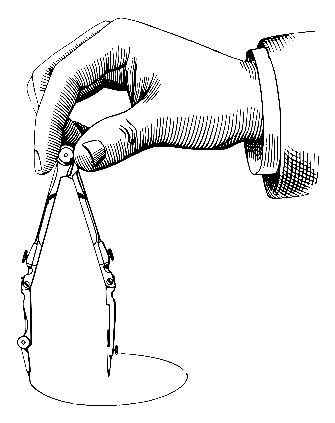
\includegraphics[height=5cm]{\currentpath/images/compas.eps}
% compas.eps: 0x0 pixel, 300dpi, 0.00x0.00 cm, bb=
\end{center}
\vfill
             % On inclut le glossaire
     
    % ============================================================================================
    % ======= Lexique
    % ============================================================================================

    \def\currentpath{./lexique/lexique}    % On définit le répertoire courant    
    % ============================================================================================
% ======= Lexique
% ============================================================================================

% ============================================================================================
% LES LIGNES SUIVANTES SERVENT ÉVENTUELLEMENT DE DOCUMENTATION
% ============================================================================================

% % Classement forcé
% % Impose le symbile int directement après le mot intégrale
% \MotDefinition{$\int$}[integrale]{symbole}
% \MotDefinition{intégrale}{mot intégrale}
% \MotDefinition{intégration}{autre mot intégrale}

% % Utilisation d’un mot au pluriel dans le texte alors que le lexique présente normalement le mot au singulier.
% % Par exemple, on utilise le code pour ajouter l'entrée au lexique :
% \MotDefinition[mot]{mots}{Exemple mot lexique distinct du texte}
% % Et comme ceci dans un texte
% Utilisation de \MotDefinition[mot]{mots}{} au pluriel dans le texte alors que le lexique présente normalement le mot au singulier.

% ============================================================================================
% On centralise les entrées du lexique ici
% Quelques définitions pour la maquette ...
% ============================================================================================

\MotDefinition{cercle inscrit}{Le cercle inscrit à un triangle est le cercle tangent aux trois côtés de ce triangle. 
Son centre est le point de concours des \Lexique{bissectrices} de ce triangle.\begin{center}\begin{tikzpicture}[general, scale=0.27] 
\draw[color=A2,fill=A2] (6.92,0.99) -- (7.32,1.11) -- (7.2,1.52) -- (6.79,1.4) -- cycle; 
\draw[color=A2,fill=A2] (9.98,0.29) -- (9.6,0.11) -- (9.78,-0.28) -- (10.16,-0.1) -- cycle; 
\draw[color=A2,fill=A2] (6.93,-4.08) -- (7.09,-3.69) -- (6.7,-3.53) -- (6.54,-3.92) -- cycle; 
\clip(-1,-7) rectangle (14,3);
\draw (-0.82,-0.9) -- (9.12,2.1) -- (13.3,-6.7) -- cycle;
 \draw [domain=6.54:7.61] plot(\x,{(--75.01-9.21*\x)/-3.78});
 \draw(7.61,-1.31) circle (2.83);
 \draw [domain=6.79:7.61] plot(\x,{(-46.76--6.48*\x)/-1.96});
\draw [domain=7.61:10.16] plot(\x,{(-28.24--2.73*\x)/5.74});
\end{tikzpicture}\end{center}}

\MotDefinition{médiane (d'un triangle)}{Dans un triangle, une médiane est un segment qui joint un sommet du triangle et  le milieu du côté opposé à ce sommet.
\begin{center}\begin{tikzpicture}[general, scale=0.9]
\draw (0,0)--(4,1)--(1,3)--cycle;
\draw[color=F1, epais] (1,3)--(2,0.5);
\draw[color=F1] (1,0.25) node {$\approx$};
\draw[color=F1] (3,0.75) node {$\approx$};
\end{tikzpicture}
\end{center}}

\MotDefinition{médiatrice}{La médiatrice d'un segment est la droite qui coupe ce segment perpendiculairement en son milieu.
La médiatrice d'un segment est un axe de symétrie de ce segment.
\begin{center}\begin{tikzpicture}[general, scale=0.9]
   \draw[shift={(2,2.5)}, rotate=-14, color=J1, fill=J1] (0,0)rectangle(0.3,0.3);
   \draw (0.5,2.825)--(3.5,2.125);
   \draw[color=J1] (1.5,0.5)--(2.5,4.5);
   \foreach \x/\y/\N/\pos in {0.5/2.825/A/left, 3.5/2.125/B/right} {\draw (\x,\y) node{$\times$};\draw (\x,\y) node[\pos]{$\N$}; } 
   \draw (2,2.5) node[below left] {$O$};
   \draw (3,4) node {$(d)$};
  \draw (1.25,2.66) node[color=A1, rotate=-19.29] {$\infty$};
  \draw (2.75,2.31) node[color=A1, rotate=-19.29] {$\infty$};
  \end{tikzpicture}\end{center}}

\MotDefinition{rationnel (nombre)}{Un nombre rationnel est un nombre qui peut s'écrire sous la forme d'une fraction de deux nombres entiers.}    % On inclut le lexique via \input cf doc sesamanuel p45
    
    % Par défaut sur deux colonnes, l'utilisation d'une seule colonne est automatiquement
    % remplacée par l'utilisation de deux colonnes
    \AfficheLexique 
    
    % \addcontentsline{toc}{chapter}{\StringCorriges \pageref{toutes-solutions}}

    \def\currentpath{./couverture}                      % On définit le répertoire courant
    \pagestyle{backCover}
\parindent=0pt
https://mathslozano.fr/ \hspace*{\stretch{1}} Master Manuel \LaTeX 

Classe sesamanuel modifiée\hspace*{\stretch{1}} Paquet ProfCollege
\vspace*{\stretch{1}}
\begin{center}
    \includegraphics[scale=0.5]{images/8.png}%
\end{center}
\vspace*{\stretch{1}}
\hrulefill

Du texte ici si je veux \ldots

\hrulefill
\vspace*{1cm}
\begin{center}\bfseries\Large
    \myAuthorName
\end{center}
    
\vspace*{\stretch{2}}
\begin{flushright}
       Le \today 
\end{flushright}   
\begin{center}
    \includegraphics[scale=0.5]{images/8.png}%
\end{center}
             % On inclut la 4e de couverture
\end{document}